\documentclass[a4paper,12pt]{article}
\usepackage{listings}
\usepackage{graphicx}
\usepackage{color}
\usepackage{afterpage}
\usepackage{amsmath}

\definecolor{lightgray}{rgb}{.9,.9,.9}
\definecolor{darkgray}{rgb}{.4,.4,.4}
\definecolor{purple}{rgb}{0.65, 0.12, 0.82}

\begin{document}

\graphicspath{ {./images/} }
\lstdefinelanguage{JavaScript}{
  keywords={typeof, new, true, false, catch, function, return, null, catch, switch, var, if, in, while, do, else, case, break},
  keywordstyle=\color{blue}\bfseries,
  ndkeywords={class, export, boolean, throw, implements, import, this},
  ndkeywordstyle=\color{darkgray}\bfseries,
  identifierstyle=\color{black},
  sensitive=false,
  comment=[l]{//},
  morecomment=[s]{/*}{*/},
  commentstyle=\color{purple}\ttfamily,
  stringstyle=\color{red}\ttfamily,
  morestring=[b]',
  morestring=[b]"
}

\lstset{
   language=JavaScript,
   extendedchars=true,
   basicstyle=\footnotesize\ttfamily,
   showstringspaces=false,
   showspaces=false,
   numbers=left,
   numberstyle=\footnotesize,
   numbersep=9pt,
   tabsize=2,
   breaklines=true,
   showtabs=false,
   captionpos=b
}

\title{Structuring asynchronous requests in AngularJS 1.3 \\ \vspace{-2 mm} {\small Blurring the line between asynchronous and synchronous code}}
\date{November 16, 2014}
\author{Peter Crona\\ IceColdCode.com}
\maketitle

\begin{abstract}
This paper presents a new tool for structuring asynchronous requests in AngularJS 1.3. The tool is
called \emph{StateDataStream}. Today it is common that developers mix data loading and data processing in a way that reduces readability and flexibility. 
This papers evalulates different ways of structuring asynchronous requests, starting with callbacks, then promises and finally the StateDataStream.
Both callbacks and promises have drawbacks, some of which StateDataStream solves. StateDataStream achieve a clarity close to that of synchronous data loading code.
\end{abstract}
\clearpage

\afterpage{\null\newpage}
\clearpage

\tableofcontents
\clearpage

\afterpage{\null\newpage}
\clearpage

\section{Background}
Two very common techniques for structuring asynchronous requests are \emph{callbacks} and \emph{promises}.
We will define these in short. Let us first look at some differences between traditional websites and \emph{single page web applications}.
This will help us to understand why data loading has become more complex as well as more important.
The figures below show how the architecture of traditional websites and single page web applications typically look.

\begin{figure}[!htbp]
  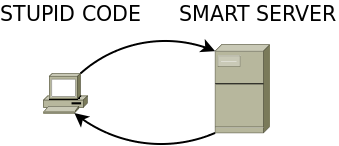
\includegraphics[scale=0.4]{traditional_cs_model.png}
  \caption{
    Traditionally the web server has contained logic and then delivered a rendered page to the user.
    The rendered page contained most, if not all data that the user requested.
  }
\end{figure}

\begin{figure}[!htbp]
  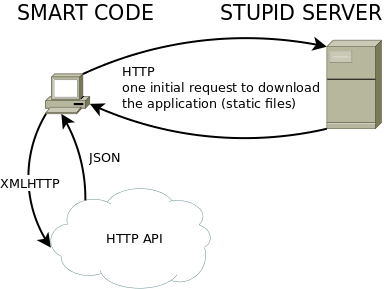
\includegraphics[scale=0.4]{new_cs_model.png}
  \caption{
    Today it is common to develop single page web applications. 
    Single page web applications can be considered being standalone applications delivered by a web server. The web server is only responsible for delivering files
    and does not contain application logic, the logic resides in the frontend and the APIs used by the frontend.
  }
\end{figure}
\clearpage
This report focuses on single page web applications. A single page web application typically contains complex data loading logic. 
For every view data needs to be loaded, where a view corresponds to a page in a traditional website. The data is sometimes dependent on other data, for instance
we might want to load information about a user and then load additional data based on the user's information. The data might also be independent, in which case
we want to load it in parallel so that we get all data as quickly as possible. 
Serverside, when using languages such as PHP or Python, data loading is handled synchronously. It might look like:

\begin{lstlisting}[caption={Code showing how data loading might look like when done synchronously}, frame=single]
user = loadUserInfo();
repos = loadUserRepos(user.githubName);
// We have both user and repos here
\end{lstlisting}
Note how clear the code is. We can read it from to to bottom and at each row we now exactly what data we have.

In JavaScript data is loaded asynchronously. This makes it easier to create rapid user interfaces and to load data in parallel. However, it comes at the price of increased complexity.
The code becomes more difficult to follow, we cannot follow the execution by reading it from top to bottom anymore.
A solution which harness the benefits of asynchronous data loading as well as the clearness of synchronous data loading is definitely desirable.
Let us have a look at the two main approaches used today, namely callbacks and promises.

\subsection{Callbacks}
The basic idea behind using callbacks is to call a method with another method as argument. When the first method has finished it will call the method you provided in the argument.
It is very simple to use, but it has some drawbacks when used for more advanced data loading. Consider this trivial example where we just send one request to get some data.

\begin{lstlisting}[caption=Code showing how we can load data using callbacks, frame=single]
Api.getUserInfoById(43, 
                    userInfoResponseHandler, 
                    errorHandler);

function userInfoResponseHandler(response) { ... }
\end{lstlisting}
Now imagine that we have two \emph{dependent} pieces of data that we want. Consider the case where part of a user's information is
his or hers Github username. After loading the user's info we want to load the user's repos on Github.

\begin{lstlisting}[caption={Code, using callbacks, showing how we can load two pieces of data, where the second is dependent on the first}, frame=single]
Api.getUserInfoById(43, 
                    userInfoResponseHandler, 
                    errorHandler);

function userInfoResponseHandler(response) {
  var githubName = response.githubName;

  // Possibly do more stuff with userInfo response here.

  Api.getGithubRepos(githubName, 
                     githubResponseHandler, 
                     errorHandler);
}

function githubResponseHandler(response) { ... }
\end{lstlisting}
This code is a quite unclear. Getting an overview of what data is loaded is difficult. If we want to do more things with the user information we will either have to mix data loading and data processing (do stuff in userInfoResponseHandler) or we
have to send all data to the githubResponseHandler and process it there. Both ways result in a quite unclear structure. It is not intuitive that the response handler for loading Github repos shall be responsible for handling user data. The structure is not a result of what we want to express, it is a result of how callbacks work. 
Clearly it has worse readability than if we would have loaded data synchronusly.
Furthermore, it is difficult to extend so that it loads more data, for example if we would want the number of contributors for the Github repos. Now let us have a look at how we could accomplish the same with promises.

\subsection{Using promises}
First a brief description of what promises are. When doing an asynchronous request, instead of you sending a callback as an argument, a so called promise is returned. The promise is an object with methods where you can register callbacks.
In AngularJS one of the most important methods of promises is `then`.
\[ then(successHandler, errorHandler) \]
Note that a promise is not just another way of specifying callbacks. For example the successHandler or errorHandler will always be called with the data as argument after it has loaded.
Even if you already called `then` before (and got the results) or if the data was loaded before you called `then`.
Now that you know a little about promises, consider the case where we just want to load one piece of data, information about a user.

\begin{lstlisting}[caption=Code showing how we can load a user's info with promises, frame=single]
Api.getUserInfoById(43)
   .then(userInfoResponseHandler)
   .catch(errorHandler);

function userInfoResponseHandler(response) { ... }
\end{lstlisting}
If we have two dependent pieces of data it might look like this:

\begin{lstlisting}[caption={Code showing an approach using promises where we are loading two pieces of data, where the second is dependent on the first}, frame=single]
Api.getUserInfoById(43)
   .then(userInfoResponseHandler)
   .catch(errorHandler);

function userInfoResponseHandler(response) {
  var githubName = response.githubName;

  // Possibly do more stuff with userInfo response here.

  Api.getGithubRepos(githubName)
     .then(githubResponseHandler), 
     .catch(errorHandler);
}

function githubResponseHandler(response) {
  ...
}
\end{lstlisting}
This is very similar to the callback method. However, there are more ways of solving the same problem with promises.
Another example where we use the possibility to chain promises is:

\begin{lstlisting}[caption={Code where we use promises and the possibility to chain promises to load two pieces of data, where the second is dependent on the first}, frame=single]
Api.getUserInfoById(43)
   .then(loadGithubRepos)
   .then(githubResponseHandler)
   .catch(errorHandler);

function loadGithubRepos(response) {
  var githubName = response.githubName;

  // Possibly do more stuff with userInfo response here.

  return Api.getGithubRepos(githubName);
}

function githubResponseHandler(response) {
  ...
}
\end{lstlisting}
Note that we have a much clearer code. By just looking at the first block of code we can see that we are getting user info, loading github repos and then handling the
response of them. But we still lack a separation of data loading and processing. One possible way of accomplishing this is:

\begin{lstlisting}[caption={Code where we chain promises together and separate data loading from data processing. However, note that we use variables in the scope outside where we load our data.}, frame=single]
var userInfo = null; var gitRepos = null;

Api.getUserInfoById(43)
   .then(loadGithubRepos)
   .then(githubResponseHandler)
   .then(processData)
   .catch(errorHandler);

function loadGithubRepos(response) {
  userInfo = response;
  return Api.getGithubRepos(response.githubName);
}

function githubResponseHandler(response) {
  gitRepos = response;
}

function processData() { Do stuff with userInfo and gitRepos }
\end{lstlisting}
But this approach have two drawbacks. Firstly, we use variables in an outside scope as storage, which can damage readability and makes it more difficult to reason about the code since the functions are less pure (rely on data not given in the parameters and have side effects).
Secondly, we treat the loading of user info differently, despite that it is just loading data just as loadGithubRepos.
Another approach without these drawbacks (I'm using Angular's \$q in this pseudo code) is:
\clearpage
\begin{lstlisting}[caption={Code where we are using promises and have separated data loading from data processing as well as made it very clear what data we are loading}, frame=single]
$q.when({})
  .then(loadUserInfo)
  .then(loadGithubRepos)
  .then(processData)
  .catch(errorHandler);

function loadUserInfo(state) {
  return Api.getUserInfoById(43).then(function(res) {
    state.userInfo = res;
    return state;
  });
}


function loadGithubRepos(state) {
  return Api.getGithubRepos(state.userInfo.githubName)
            .then(function(res) {
               state.githubRepos = res;
               return state;
            });
}

function processData(state) {
  console.log(state.userInfo);
  console.log(state.githubRepos);
}
\end{lstlisting}
By just looking at the chain of promises we can directly see that we are loading user info, then github repos and finally we process the data.
All data loading is treated the same. We can easily add more `loaders` if we need to load more data. The clarity that we have is not that far from the clarity of synchronous data loading.
However, this solution is not perfect. It is unclear what loadUserInfo does, we need to look at the actual function to know that it writes to `userInfo` in the state. When loading data
synchrnously we easily see which variable we assign the value to. Another issue is that it is unclear that loadGithubRepos must be after loadUserInfo. We need to look at both loadUserInfo and loadGithubRepos to know that there
is a dependency between them. Furthermore, if we would like to load independent data this would not be done in parallel. 
StateDataStream currently attacks that it is unclear where in the state functions are writing (to which property) and that data is not loaded in parallel even if independent.
The problem with the unclear dependencies in the chain of promises is discussed in section \ref{sec:future}.

\clearpage

\section{The StateDataStream way}
StateDataStream is solving the problem that it is unclear where the result of a promise is written when multiple promises are chained together. 
It also makes it easy to run independent AJAX-requests in parallel. Since the syntax is quite clear let us start with an example:

\begin{lstlisting}[caption={Code showing how two pieces of data, where the second is dependent on the first, can be loaded using StateDataStream.}, frame=single]
StateDataSteam.init({})
  .write('userInfo', Api.getUserInfoById(43))
  .write('githubRepos', function(state) {
     return loadGithubRepos(state.userInfo.githubName);
  })
  .error(errorHandler)
  .execute(proceessData);

function processData(state) {
  console.log(state.userInfo);
  console.log(state.githubRepos);
}
\end{lstlisting}
We have achieved a clear separation between data loading and data processing. Furthermore, it is clear where we are writing the results of promises. `userInfo` and other promises directly added to the stream (i.e. not wrapped in a function) will be sent in parallel as soon as we add them to the stream. Hence loading independent data in parallel is easy and does not damage the readability of the code.
The clarity of the code is compareable with synchronous data loading. The code can be read from top to bottom and we can easily see to which `variables` results are assigned.

Now let us have a look at the details of StateDataStream, how we specify what data to load and how to handle errors. And finally also how to execute the stream, making it possible for us to use all the data we have written into the state.

\subsection{Specifying the stream}
Initially we just specify the stream. The idea is that nothing we do should have side effects. However, as you may have noted, promises directly written to the
stream will be sent immediately, since the parameters of functions are evaluated directly. Fortunately, due to how promises work, we can disregard from this. 
The following sub sections will describe the operations available for specifying the stream.

\subsubsection{Writing to the stream}
As you have seen we can write different things to the stream. A semi-formal description of the write operation is:
\[ write(key, val) \]
where
\begin{flalign}
\begin{aligned}
val &:= value\ |\ promise\ |\ function \nonumber \\
key &:= objectRef\ |\ listRef \nonumber
\end{aligned}
\end{flalign}
\emph{objectRef} and \emph{listRef} use dot notation to specify where to put the key. Both use the same syntax except that listRef always end with []. An example will suffice to describe their syntax:
\newline

\begin{lstlisting}[caption=Examples of listRef and objectRef keys, frame=single]
StateDataSteam.init({})
  .write('userInfo', val) // objectRef
  .write('user.info', val) // objectRef
  .write('user.says.hello', val) // objectRef
  .write('users[]', val) // listRef
  .write('data.users[]', val); // listRef

  // Let ? symbolise any data, then the state will look like:
  {
     userInfo: ?,
     user: {
       info: ?,
       says: {
         hello: ?
       }
     },
     users: [?],
     data: {
       users: [?]
     }
  }
\end{lstlisting}
We also need to define \emph{function} a little more. A function is just an ordinary function, but it may return a promise, in which case the promise will be resolved and written to
the stream. And if a value (anything except a promise) is returned, the value will be written to the stream.

\subsubsection{Error handling}
A stream is associated with one error handler. The error handler will immediately be called if some HTTP-request returns another status than 200. Meaning that any subsequent
operations will not be carried out. The error handler is called with the error and the state at the time of the error as arguments.
\[ errorHandler(error, state) \]

The error handler is associated with the stream in the following way:
\begin{lstlisting}[caption=Attaching an error handler to the stream, frame=single]
StateDataSteam.init({})
  .write('userInfo', val)
  .error(errorHandler);
\end{lstlisting}
Now let us move on to actually doing something with the stream, i.e. executing it.

\subsection{Executing the stream}
Once the stream is specified it can be stored in a variable or you might create a function which returns the stream parameterised by some arguments.
Regardless of which, the way to execute the stream is simply to call execute:

\begin{lstlisting}[caption=Executing the stream, frame=single]
StateDataSteam.init({})
  .write('userInfo', val)
  .error(errorHandler)
  .execute(initController);
\end{lstlisting}
The function initController will be called with the resulting state of running the stream, assuming that an error is not detected, in which case the error handler will be called instead. 
The handler initController shall have the following signature:
\[ initController(state) \]
and in this case state will just be an object containing the property \emph{userInfo}. Note that the state is completely defined by the inital state and what we write to the state.
By just looking at the stream specification we get a good image of what will be available in initController.

\section{Conclusion and future considerations}
\label{sec:future}
StateDataStream provides a new way of structuring asynchronous requests. It separates data loading from data processing and it has a very clear syntax, which makes it easy to see 
what data is loaded and how to access it in the data processing step. The data loading code's clarity is compareable with synchronous data loading.
Furthermore, it is easy to load independent data in parallel and it is easy to specify one 
error handler for the whole stream. It solves some of the drawbacks with callbacks and promises, which are commonly used today. However, it does not yet support making it easy to indentify dependencies between write operations nor loading dependent data in parallel
in an easy way.

\subsection{Specifying dependencies between writes}
\label{sec:spec_dependencies}
Consider the following piece of code:

\begin{lstlisting}[caption=Executing the stream, frame=single]
StateDataSteam.init({})
  .write('users[]', Api.getUsers())
  .write('githubRepos[]', function(state) {
     // Load github repos for all users
  })
  .error(errorHandler)
  .execute(initController);
\end{lstlisting}
It is not obvious that gitHubRepos depends on the data in state.users. We need to look at the code. If the function for loading data is not specified inline (with an anonymous function) this will significantly damage readability.

One possible way to make dependencies more clear is to introduce a third parameter for the write method. In that case we might get something like:

\begin{lstlisting}[caption=Executing the stream, frame=single]
StateDataSteam.init({})
  .write('users[]', Api.getUsers())
  .write('githubRepos[]', loadGithubRepos, ['users']);
\end{lstlisting}
In the code above it is clear that githubRepos depend on users. Furthermore, loadGithubRepos does not need to be called with the full
state, it can be called with only the specified dependencies.

\clearpage

\subsection{Running state dependent writes in parallel}
Consider the following code:
\begin{lstlisting}[caption=Executing the stream, frame=single]
StateDataSteam.init({})
  .write('users[]', Api.getUsers())
  .write('githubRepos[]', function(state) {
     // Load github repos for all users
  })
  .error(errorHandler)
  .execute(initController);
\end{lstlisting}
Currently there is no easy way of loading github repos for all users in parallel. It might be doable using \$q.all in the write. But it might be worth investing some time into investigating 
the best approach for this. One possible way to simplify this might be:

\begin{lstlisting}[caption=Executing the stream, frame=single]
StateDataSteam.init({})
  .write('users[]', Api.getUsers())
  .writeAll('githubRepos[]', loadGithubRepos, 'users')
  .error(errorHandler)
  .execute(initController);
\end{lstlisting}
Where \emph{writeAll} would cause loadGithubRepos to be called once for every element in users, and the results would be pushed into githubRepos, in parallel of course.

\subsection{Execute handlers with limited state}
It might not always be desireable to have one handler for the whole state. For instance, if we are loading user info and github repos, we might want one handler to
handle the user info and another the github repos. One idea of how this might be supported is:

\begin{lstlisting}[caption=Executing the stream, frame=single]
StateDataSteam.init({})
  .write('users[]', Api.getUsers())
  .write('githubRepos[]', loadGithubRepos, ['users'])
  .execute(userHandler, ['users'])
  .execute(githubHandler, ['users', 'githubRepos']);
\end{lstlisting}

Where userHandler would be called as userHandler(users) and githubHandler would be called as githubHandler(users, githubRepos).

\end{document}
